\documentclass[a4paper, 11pt]{article}

% packages
\usepackage[utf8]{inputenc}
\usepackage{amsmath}
\usepackage{amsfonts}
\usepackage{array}
\usepackage{booktabs}
\usepackage{chngcntr}
\usepackage{colortbl}
\usepackage{dcolumn}
\usepackage{floatrow}
\usepackage{geometry}
\usepackage{graphicx}
% \usepackage[dvipdfmx]{graphicx}  これはうまくいかない. 
\usepackage{hyperref}
\usepackage{multirow}
\usepackage{natbib}
\usepackage[normalem]{ulem}
\usepackage{ntheorem}
\usepackage{pdflscape}
\usepackage{rotating}
\usepackage{setspace}
\usepackage{subfigure}
\usepackage{tabularx}
\usepackage{threeparttable}
\usepackage[numbib, nottoc, notlot, notlof]{tocbibind}
\usepackage{wrapfig}
\usepackage{xcolor}

% page styling
\geometry{
  a4paper,
  left=1in,
  right=1in,
  bottom=1.2in,
  top=1.2in
}
\pagestyle{plain}
\pagenumbering{arabic}
\linespread{1.5}
\hypersetup{
  colorlinks,
  linkcolor={red!50!black},
  citecolor={blue!50!black},
  urlcolor={blue!80!black}
}

\title{Youth Underrepresentation and Parties' Nomination Strategy in Mixed-Member Electoral Systems}

\author{Dai Sasaki \thanks{Graduate Schools for Law and Politics, The University of Tokyo}}

\date{
	First Version: 28 Jun, 2024 \\
	This Version: 28 Jun, 2024 
}

\begin{document}

\maketitle

\begin{abstract}  % TODO: fix
Proportional representation (PR) electoral systems generally promote minority representation, including youth representation. Given this representational advantage of PR systems, the case of Japan that has a mixed member system poses a puzzle regarding the relationship between electoral systems and youth representation. This paper argues that the interaction between the two tiers of the system, dual listing, contributes to the underrepresentation in the country. Under dual listing, parties face a tradeoff between giving second chances to their members and nominating new candidates, where the former choice dominates the latter because of parties' post-election objectives. I show that parties place dual-listed candidates, senior members, and incumbents higher on the list. Furthermore, senior politicians and incumbents are more likely to be dual-listed. Given that novices are younger than the average candidate and MP, youth underrepresentation would have been mitigated without dual listing. 
\end{abstract}

\newpage

\section{Introduction}

Young citizens are underrepresented in democracies across the globe. Table \ref{table:intl} shows the age demographics of lower houses in the G7 countries. The average age of the house members exceeds 45 years old in all countries. While the median age of population exceeds 45 years old only in Italy (47.3) and Japan (48.7) \citep{un2022}, no country has more than 50 \% of legislators under 45 years old. Policy output from parliaments with biased age composition does not reflect citizens' preferences. Since voters of different age groups consider different issues to be salient, youth underrepresentation could pose a serious problem of unresponsiveness. 

\begin{table}[htbp]
\begin{center}
\begin{threeparttable}
% latex table generated in R 4.1.0 by xtable 1.8-4 package
% NOTE: manually modified on 27 Nov 2023. 
% Sat Jul  8 06:31:47 2023
\begin{tabular}{lccccc}
\toprule
Country & Eligibility & Average & \% U30 & \% U40 & \% U45 \\ 
\midrule
Canada & 18 & 50 & 1.95 & 16.88 & 30.19 \\ 
France & 18 & 49 & 4.85 & 26.52 & 37.95 \\ 
Germany & 18 & 47 & 8.83 & 28.94 & 41.98 \\ 
Italy & 25 & 49 & 1.25 & 16.25 & 35 \\ 
Japan & 25 & 55 & 0.22 & 6.02 & 17.2 \\ 
UK & 18 & 51 & 3.69 & 21.69 & 34 \\ 
USA & 25 & 57 & 0.46 & 10.42 & 20.14 \\ 
\bottomrule
\end{tabular}

\begin{tablenotes}[flushleft]
  \scriptsize{
    \item{\textit{Note.} Age demographics of lower house members in the G7 countries, as of January 2023. Eligibility is the minimum age to run for the house.}
    \item{\textit{Source.} \citet{ipu2023}.}
  }
\end{tablenotes}
\end{threeparttable}
\caption{Age Demographics of Lower Houses in the G7 Countries}
\label{table:intl}
\end{center}
\end{table}

There are mainly two strands of research on youth underrepresentation, but neither specifies its causes or provides detailed explanations of its mechanisms. The first type of study exploits conjoint experiments to study voter preferences of candidates' age \citep{eshima2022just, horiuchi2020identifying, mcclean_too_2024}. These studies find no evidence that voters discriminate against young candidates. Instead, they are as favorable toward young candidates as middle-aged politicians and prefer them to elderly candidates. The other class of studies explores factors conditioning legislators' age through cross-national analyses \citep{joshi2013representation, stockemer2018age, stockemer_youth_2022, stockemer_age_2023}. 
% TODO: more detail
Among these studies, \citet{joshi2013representation} shows that the proportion of young legislators is higher in countries with proportional representation (PR) electoral systems than in those with majoritarian systems, a finding consistent with prepositions on the relationship between electoral systems and minority representation (e.g., \citet{norris_electoral_2004}). However, we are yet to understand how specific electoral rules affect the behavior of actors within the system, thereby preventing young candidates from entering the legislature. 

The case of Japan poses a puzzle regarding the relationship between electoral systems and youth representation. Japan introduced a mixed member (MM) electoral system after the 1994 electoral reform, which combines two electoral tiers based on majoritarian and PR formulae. The Lower House of the Japanese Diet (House of Representatives; HoR) severely underrepresents young voters. It has only seven percent of legislators under 40 as of 2018, the fewest among G7 countries and third-fewest among 37 OECD countries \citep{mcclean2020thesis}. Interestingly, even though the HoR election has majoritarian districts and PR blocks, candidates and winners in the PR tier are similarly aged to those from the majoritarian tier. 

This paper shows that the representational benefits of PR electoral systems could be reduced under some forms of mixed-member systems. Specifically, I claim that the nomination option of ``dual listing" in Japan's lower house election incentivizes parties to give second chances to their existing members, thereby limiting the number of new candidates they nominate. Japan's lower house election allows parties to nominate candidates simultaneously in a single-member district (SMD) and a PR block (``dual listing"). Dual-listed candidates have a second chance of election in the PR tier, even if they fail to win in the SMD tier. This institutional device allows parties to give ``second chances" to their candidates. 

In general, parties prioritize senior politicians over junior members in nominations. Parties attempt to maximize not only the number of votes they obtain in the election but also post-election gains, such as policies and ministerial posts. Senior politicians are better suited for the latter objectives, as they possess more political resources. For example, they may have developed stronger ties with their constituencies through their legislative careers and, as a result, might be more effective in policy-making. 

When dual listing is allowed, parties face a trade-off in candidate nomination for the PR tier. They have two choices: the first is to give an insurance ticket to candidates in the majoritarian tier, and the other is to nominate new candidates. Since they have limited resources and cannot increase the number of nominees infinitely, they first estimate an obtainable number of seats and then allocate these winnable seats to candidates. When parties are motivated to give second chances to their existing candidates, it prevents the entry of new candidates through the PR tier, and the representational advantages of having a PR electoral system are diminished. Importantly, this happens even if parties are not biased against young candidates. They may also have incentives to appeal to younger voters by nominating young candidates, but institutional settings could encourage them otherwise. 

Analyzing the nomination patterns of PR candidates in the Japanese lower house elections between 1996 and 2017, I find that dual-listed candidates, senior candidates, and incumbents tend to be placed higher on the PR list than others. I also show that senior candidates and incumbents are more likely to be dual-listed than others. Absent the dual listing, parties do not face a trade-off between existing and new candidates in nomination, and the entry of new candidates through the PR tier would have been facilitated. Since novel candidates and legislators are generally younger than the average candidate and MP, the problem of youth representation would have been mitigated. 

PR systems are generally better suited to promoting minority representation than majoritarian systems. Youth representation is no exception: cross-national comparisons show that countries with PR systems have more young MPs than those with majoritarian systems (e.g., \citet{joshi2013representation}). However, this benefit crucially depends upon the parties' nomination strategies. The reason why PR promotes minority representation is that parties need to appeal to a broader set of voters and adjust their nomination strategies so that their PR lists include candidates with various backgrounds. However, this representational advantages can be lost without proper institutional designs under MM systems. 

This paper proceeds as follows. Section \ref{sec: the} discusses the theoretical backgrounds of the research and presents the main argument and corresponding hypotheses. Section \ref{sec: emp} presents the data and empirical strategies. Section {sec: res} shows the result of the analysis. Section \ref{sec: dis} complements the preceding section with additional empirical evidence and discusses the implication of the result for various topics of comparative politics. 

\section{Theory} \label{sec: the}

\subsection{The Absence of Research on Minority Representation Under Mixed-Member Systems}

It is well acknowledged that proportional representation (PR) electoral systems are generally better-suited than majoritarian systems in promoting minority representation \citep{matland_contagion_1996, matland_womens_1998, meserve_gender_2020}. The representational advantage of PR systems comes from how voters evaluate candidates under the PR electoral rule and how parties respond to it \citep{norris_electoral_2004}. Under PR systems, voters do not vote for a single candidate but for a list of candidates. Under such circumstances, voters decide to vote for a particular list because it contains a certain type of candidate or vice versa. For example, female voters may vote for a party list that includes a female candidate or decline to vote for a list that does not include any women. Parties, on the other hand, would want to garner votes from broader parts of the constituency. Therefore, they have incentives to include candidates with various backgrounds and labels in their lists so that they appeal to a wider set of voters. 

PR systems may promote youth representation in a similar vein. Several cross-national studies show that countries with PR systems have a larger share of young MPs than countries with majoritarian systems. \citet{joshi2013representation} compares 14 Asian lower houses and finds that legislatures with larger shares of PR seats have higher proportions of legislators under age 40. Similarly, \citet{stockemer_youth_2022} compares 129 democracies worldwide and shows that countries with PR systems tend to have more legislators under age 35 and 40. 

Given the above discussion, one might expect mixed-member (MM) electoral systems to exhibit a medium size of representational benefits compared to majoritarian and PR systems, the two ``extreme" electoral systems \citep{blais_electoral_1996, reynolds_electoral_2005, shugart_mixed-member_2003}. Mixed-member systems are often expected to deliver the ``best of the both worlds" \citep{hirano_policy, shugart_mixed-member_2003}. Specifically, scholars consider MM systems effective in moderating the extremities of the two pure systems. On the inter-party dimension, MM systems balance vote and seat shares by combining the majoritarian element that produces two-party systems and proportionality that helps smaller parties. On the intra-party dimension, they preserve and cultivate the ties between candidates and constituencies via the nominal tier while increasing party cohesion via the list tier. Similarly, one might also want to locate MM systems in the center of the spectrum of electoral systems in terms of their representational benefits. 

However, it is not certain how the representational advantages of having a PR tier function under mixed systems. Few studies are focusing on MM systems that consider minority representation (see \citet{kerevel2019mixed} for an exception), and no study has considered youth representation separately. Neither is it sure that a PR ``tier" works the same as a PR ``system". A large body of literature has explored ``contamination" in mixed systems, a class of spillover effects of one tier on the other \citep{cox_interaction_2002, ferrara_mixed_2005, herron_contamination_2001, nishikawa_mixed_2004, moser_mixed_2004}. The primary concern of these studies is the consequences of contamination on party systems, especially on how the number of parties or candidates under mixed systems differs from the theoretical expectations of Duverger's Law. Some scholars investigate parties' nomination strategies under mixed systems \citep{ferrara_going_2005}. However, their focus is on the inter-party dimension (i.e., electoral coordination), not the intra-party dimension, where the dynamic relationship between voters and parties could help minority candidates represented. 

\subsection{Japan's Case: MM System with Interaction}

The case of Japan provides an interesting puzzle in considering youth representation under mixed-member systems. Japan introduced a mixed-member system combining single-member districts (SMDs) and closed-list PR blocks as a result of the electoral reform in 1994. Under the new electoral system, each voter has two votes and casts one for an SMD candidate and the other for a party list. SMD winners are determined by the ``first-past-the-post" rule; PR seats are first distributed to parties by the D'Hondt method and then to candidates according to the list rank. A party's total number of seats is the sum of the seats it won in the two tiers. Thus, Japan's mixed-member system falls into the category of the ``mixed-member majoritarian (MMM)", as compared to ``mixed-member proportional (MMP)," where a party's vote share in the PR tier determines the number of seats it obtains \citep{shugart_mixed-member_2003}. 

While the extent to which its lower house underrepresents young citizens constitutes an important problem itself, the puzzle is that the two tiers of its mixed-member system elect candidates of similar ages. Figure \ref{fig:pr_vs_smd} compares the age compositions of legislators elected from the majoritarian and PR tiers in the lower house election. Two distributions have similar shapes, with middle-aged legislators most common. Although the PR tier has slightly higher proportions for those aged 20 to 35, the SMD tier has a higher proportion for those aged 35 to 40. 

\begin{figure}[!htbp]
	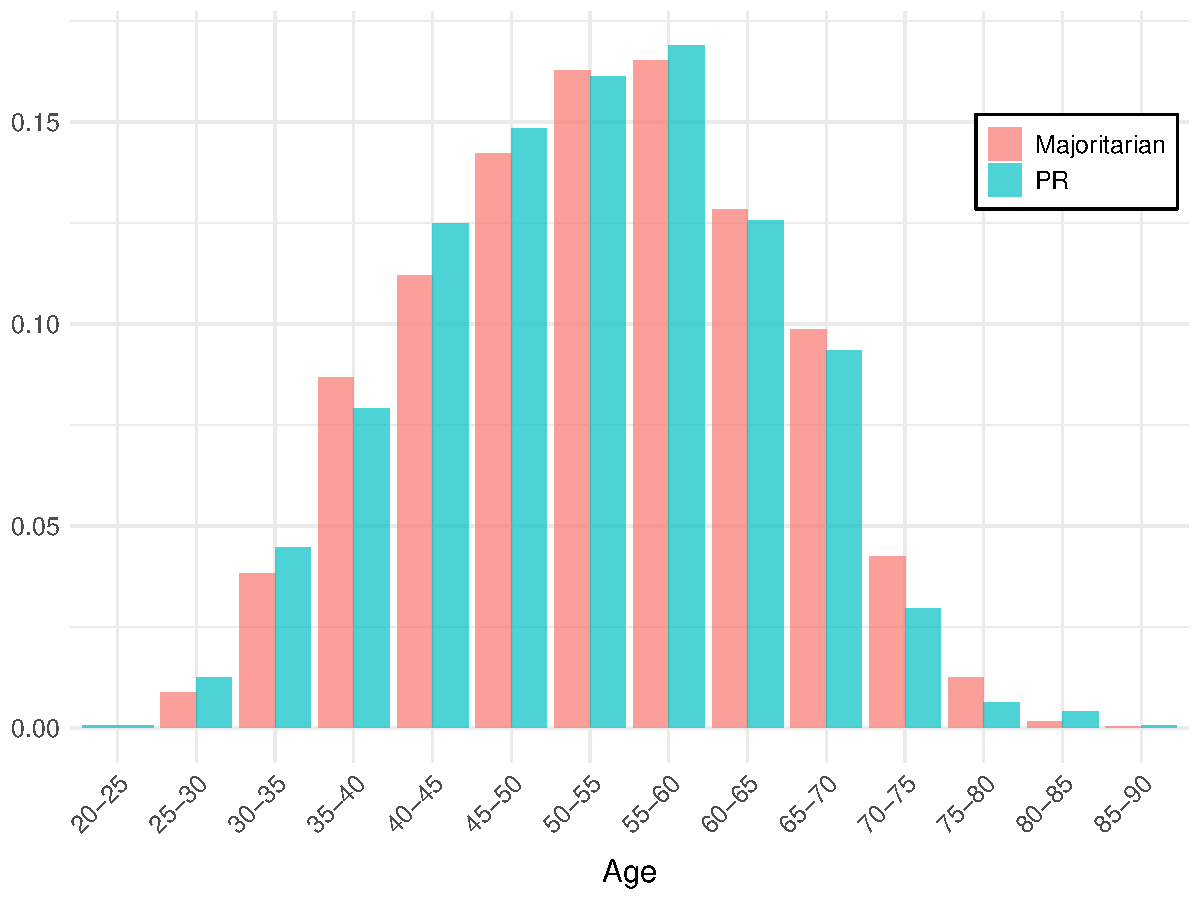
\includegraphics[width = 0.9\textwidth]{../figure/paper/age_smd_vs_pr_winners.pdf}
	\caption{Age Composition of Legislators Elected from the Two Tiers}
	\label{fig:pr_vs_smd}
\end{figure}

Interestingly, Japan's mixed-member system allows an interaction between the two tiers by adopting what is called ``dual listing" \citep{matland_determinants_2004, pekkanen2006electoral, reed2022}. Under dual listing, parties can nominate candidates simultaneously in the two tiers and give the same list rank to any of the dual-listed nominees. When the result is tallied, dual-listed candidates who won in the SMD tier are removed from the list, and those sharing the same rank are reranked according to the best-loser formula.\footnotemark{} The use of this nomination option is common: Figure \ref{fig:dual} shows the share of dual-listed nominees among PR winners in the elections between 1996 and 2017. Since the 2000 election, more than half of the PR-elected legislators are ``zombies", i.e., dual-listed candidates \citep{pekkanen2006electoral}. After 2000, the two largest parties in the post-reform era, the dominant Liberal Democratic Party (LDP) and the second largest Democratic Party of Japan (DPJ), succeeded by the Constitutional Democratic Party (CDP), have over 50 \% of zombie legislators most of the time. Komeito, the coalition partner of LDP, is an exception to this trend, as it has not used dual listing since the millennium. However, one can reasonably say that dual listing is a popular option in candidate nomination for the PR tier in post-reform Japanese politics. 

\footnotetext{Technically, candidates are reranked according to what is called ``close-loss rate". Let $i$ be a SMD-losing dual-listed candidate in the district $d$. Candidate $i$'s close loss rate, $\text{Loss}_{i}$, is calculated as 
  \[
    \text{Loss}_{i} = \frac{\text{Vote}_i}{\text{max}(\text{Vote}_d)}, 
  \]
\noindent where $\text{max}(\text{Vote}_d)$ denotes the largest number of votes obtained in the district $d$ (i.e., that of the winner). 
} 

\begin{figure}[!htbp]
	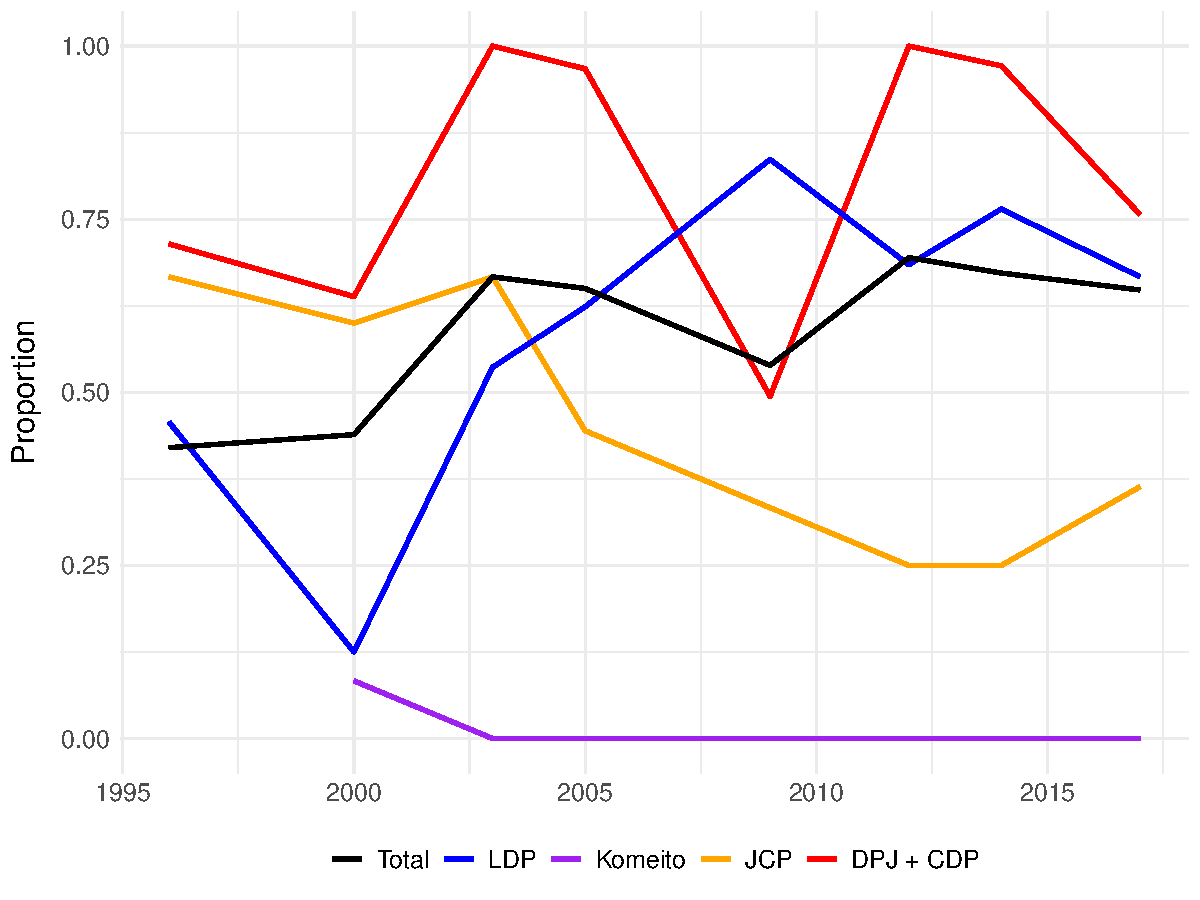
\includegraphics[width = 0.9\textwidth]{../figure/paper/dual_nomination.pdf}
	\caption{Share of Dual-Listed Candidates among PR Winners}
	\label{fig:dual}
\end{figure}

\subsection{Hypothesis: Dual Listing Exacerbates Youth Underrepresentation}

To answer the puzzle, I focus on the dual listing option explained in the previous subsection. Specifically, I claim that dual listing incentivizes parties to give ``second chances" to their senior members and incumbents, and that, in turn, prevents the entry of younger candidates via the PR tier. Youth representation in parliament depends on two factors: one is how many new legislators enter the legislature, i.e., how often legislative turnover occurs, and the other is at what age they win the election for the first time. Under dual listing, parties allocate PR tickets to existing members over new candidates, and that limits the number or electoral prospects of younger candidates in the PR tier. 

It is important for parties to maximize the number of votes and seats they obtain in the election, but what is as critical is to whom they give the obtained seats. Parties are not vote-garnering devices active only during the election; they also have goals at the post-election stage. Consider a policy-oriented party that aims to realize its desired policies \citep{strom_policy_1999}. It is desirable that party members possess various resources to achieve the goal: the ability to plan and legislate policies, knowledge about the legislative process, skills for negotiations, coordination with bureaucracy, and connections with stakeholders. Politicians acquire these resources as they serve as members of parliament, and it is reasonable to assume a positive relationship between their years in office and the amount of resources they have. Similarly, incumbents are better-equipped than non-incumbents with the latest knowledge and information and would be more evaluated by the party. 

If parties assign priority based on seniority and incumbency among members, they should reflect that priority in their nomination strategy. Dual listing gives parties incentives to do so: they can give ``insurance tickets" to senior members and incumbents by taking that option. The values of the insurance are heterogeneous: some candidates are placed at the top of the list, while others are given a lower rank, which is shared with other dual-listed candidates. Under the close-list PR, candidates with a higher list rank have a higher electoral prospect. 

Under dual listing, parties have two competing options in candidate nomination for the PR tier: giving second chances to candidates running in the SMD tier and nominating new candidates as pure-PR candidates. These options constitute a trade-off because the number of candidates they can nominate is finite. Firstly, the amount of parties' resources, such as financial and logistic support for candidates, is limited. Secondly, parties do not nominate far more candidates than the expected number of seats they could obtain in the election. Therefore, the number of newly nominated candidates decreases when parties dual-list existing members to give them higher electoral prospects. 

Given the above discussion, I argue that parties give second chances to their senior members and incumbents using dual listing. Specifically, I present the following five hypotheses. 

\begin{enumerate}
	\item[H1] Senior candidates are more likely to be dual-listed; 
	\item[H2] Incumbents are more likely to be dual-listed; 
	\item[H3] Senior candidates are placed higher on the list; 
	\item[H4] Incumbents are placed higher on the list; 
	\item[H5] Dual-listed candidates are placed higher on the lists. 
\end{enumerate}

\section{Data and Method} \label{sec: emp}

To test the above hypotheses, I use the Japanese House of Representatives Elections Dataset (JHRED; \citet{reedsmith2018}). Specifically, I analyze the nomination patterns of candidates running in the PR tier of the post-reform general election between 1996 and 2017. This criterion leaves 6,935 candidates across eight elections (2000, 2003, 2005, 2009, 2012, 2014, 2017). Table \ref{tab:stats} in the appendix presents candidate-level summary statistics.

For Hypotheses 1 and 2, I estimate logistic models that regress the dual listing dummy on the explanatory variable, the number of a candidate's past elections in the lower house elections, or the incumbency dummy, along with a set of covariates. I proxy candidates' seniority with the number of their past wins because politicians' seniority is measured by the number of terms they served in the same house \citep{pekkanen2006electoral}. The covariates include the female dummy, district magnitudes, and two-way fixed effects of election year and party. I control for candidates' gender because parties have incentives to give female candidates to appeal to a broader set of voters \citep{salmond2006proportional, chiru2017value}. I also account for block magnitudes, as the length of a list partially depends on the maximum number of candidates elected. Magnitudes vary across time and region: see Table \ref{tab:distM} in the appendix for details. Party fixed effects are supposed to account for different nomination patterns among parties. For example, \citet{fujimura2012position} finds different patterns for LDP and DPJ in allocating the parties' important positions. Given party-level variations in the candidate evaluation, it is reasonable to assume party-specific patterns of candidate nomination. For Hypotheses 3 and 4, I estimate negative binomial models that regress candidates' list rank on the explanatory variable and the same set of covariates. The application of negative binomial models is intended to account for the fact that the distribution of list rank is extremely right-skewed: see Figure \ref{fig:distRank} in the appendix for details.

\section{Result} \label{sec: res}

Table \ref{tab:reg} presents the result of the regression analysis. All of the five hypotheses are supported after controlling for potential confounders. I find that the number of candidates' past elections and incumbency status are positively correlated with whether they are dual-listed in the PR tier. Candidates with more past elections and incumbents tend to be placed higher on the party list. These relationships hold regardless of candidates' gender, affiliated party, district magnitude, and election year. 


\begin{table}
\begin{center}
\begin{tabular}{l c c c c c c c c c c}
\hline
 & \multicolumn{4}{c}{List Rank} & \multicolumn{3}{c}{Dual Listing} & \multicolumn{3}{c}{Dual Listing (Tie)} \\
\cline{2-5} \cline{6-8} \cline{9-11}
 & Model 1 & Model 2 & Model 3 & Model 4 & Model 5 & Model 6 & Model 7 & Model 8 & Model 9 & Model 10 \\
\hline
Total Wins         & $-0.15^{***}$ &               &               & $-0.10^{***}$ & $0.16^{***}$ &              & $-0.00$      & $0.14^{***}$ &              & $0.00$        \\
                   & $(0.01)$      &               &               & $(0.02)$      & $(0.04)$     &              & $(0.02)$     & $(0.04)$     &              & $(0.02)$      \\
Incumbency         &               & $-1.02^{***}$ &               & $-0.74^{***}$ &              & $1.33^{***}$ & $1.33^{***}$ &              & $1.16^{***}$ & $1.13^{***}$  \\
                   &               & $(0.12)$      &               & $(0.11)$      &              & $(0.28)$     & $(0.28)$     &              & $(0.32)$     & $(0.31)$      \\
Dual Listing       &               &               & $-1.82^{***}$ & $-0.93^{***}$ &              &              &              &              &              &               \\
                   &               &               & $(0.25)$      & $(0.27)$      &              &              &              &              &              &               \\
Tie                &               &               &               & $-1.92^{*}$   &              &              &              &              &              &               \\
                   &               &               &               & $(0.86)$      &              &              &              &              &              &               \\
Female             &               &               &               & $-0.07$       &              &              & $-0.24^{*}$  &              &              & $-0.40^{***}$ \\
                   &               &               &               & $(0.04)$      &              &              & $(0.12)$     &              &              & $(0.11)$      \\
Block Magnitude    &               &               &               & $0.02^{***}$  &              &              & $0.04^{***}$ &              &              & $0.04^{***}$  \\
                   &               &               &               & $(0.01)$      &              &              & $(0.01)$     &              &              & $(0.01)$      \\
Total Wins x Tie   &               &               &               & $0.10^{***}$  &              &              &              &              &              &               \\
                   &               &               &               & $(0.02)$      &              &              &              &              &              &               \\
Tie x Incumbency   &               &               &               & $0.49^{**}$   &              &              &              &              &              &               \\
                   &               &               &               & $(0.18)$      &              &              &              &              &              &               \\
Tie x Dual Listing &               &               &               & $0.84$        &              &              &              &              &              &               \\
                   &               &               &               & $(0.91)$      &              &              &              &              &              &               \\
\hline
Year FE            & Yes           & Yes           & Yes           & Yes           & Yes          & Yes          & Yes          & Yes          & Yes          & Yes           \\
Party FE           & Yes           & Yes           & Yes           & Yes           & Yes          & Yes          & Yes          & Yes          & Yes          & Yes           \\
AIC                & $37167.39$    & $36446.03$    & $33098.42$    & $31652.57$    & $5886.23$    & $5697.89$    & $5629.09$    & $5949.29$    & $5803.79$    & $5729.36$     \\
Log Likelihood     & $-18536.69$   & $-18176.02$   & $-16502.21$   & $-15771.28$   & $-2897.12$   & $-2802.94$   & $-2765.54$   & $-2928.64$   & $-2855.90$   & $-2815.68$    \\
Num. obs.          & $7754$        & $7754$        & $7754$        & $7754$        & $7754$       & $7754$       & $7754$       & $7754$       & $7754$       & $7754$        \\
\hline
\multicolumn{11}{l}{\scriptsize{\item $^{***}p<0.001$; $^{**}p<0.01$; $^{*}p<0.05$. Standard errors clustered at the party level in parentheses.
\item Dependent variable: candidate $i$'s list rank (columns 1-4) dual listing status (columns 5-7), and whether the candidate has a tie on the list (columns 8-10).
\item Estimated models: negatige binomial (columns 1-4) and logit (columns 5-10).}}
\end{tabular}
\caption{Regression Results}
\label{tab:regression_results}
\end{center}
\end{table}


To illustrate these results within a specific context, I present several marginal effects plots. Using a hypothetical candidate profile, I modify the candidate's characteristics and examine the corresponding changes in the probability of being dual-listed and list rank. Specifically, the benchmark candidate is a male candidate affiliated with LDP, running in the Tokyo block in the 2012 election, which has the median block size of 17. Figure \ref{fig:dual} presents the predicted probabilities of the candidate being dual-listed, according to his incumbency status and the number of his previous wins in the election. Although the baselines are quite high, he is predicted to be significantly more likely to be dual-listed when he is a returning candidate or a candidate with past legislative experience. Specifically, the probability of dual listing is higher by more than ten percent when he is an incumbent. The relationship between seniority and dual-listing status is nonlinear, but he is about 10 percent more likely to be dual-listed when he has been elected five times compared to when he is a novice. 

\begin{figure}[!htbp]
	\caption{Dual Listing and Incumbency (Left); Seniority (Right)}
	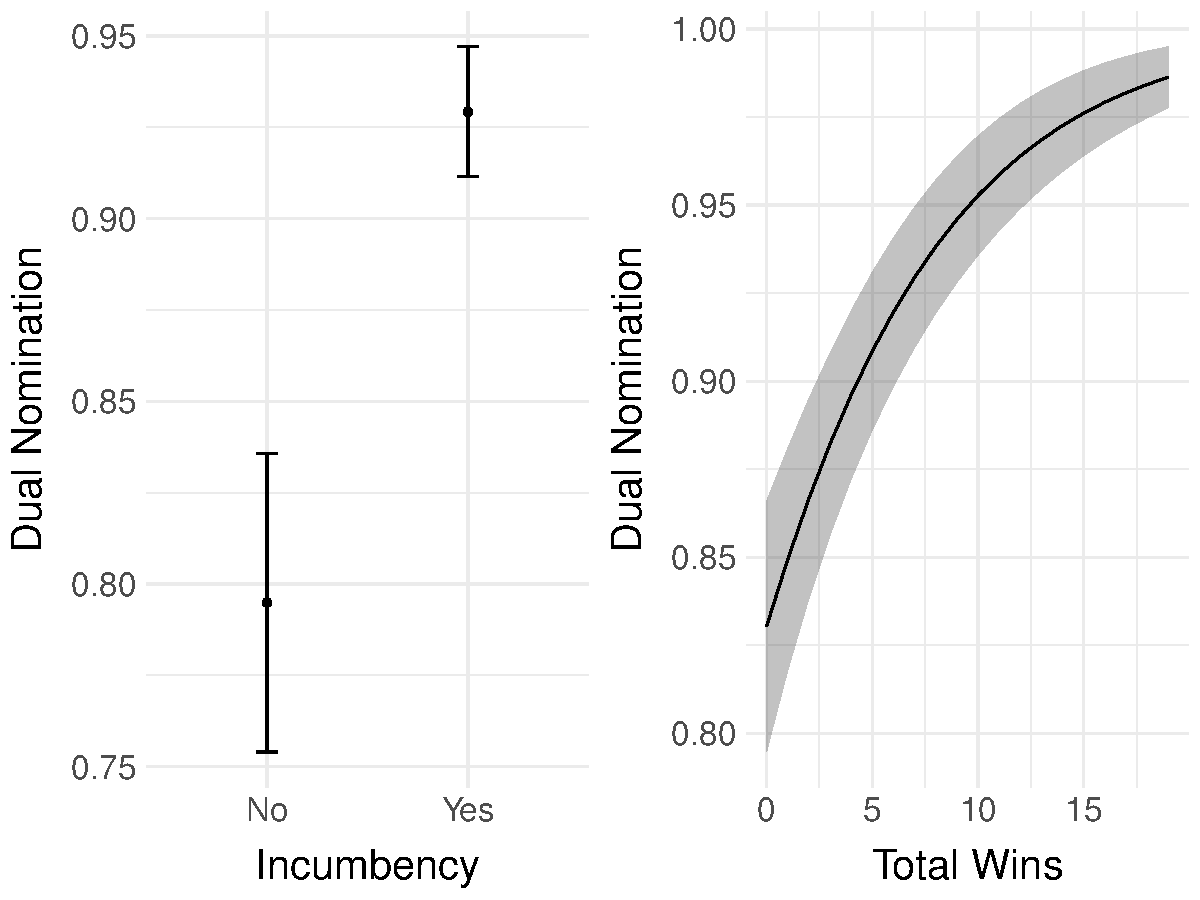
\includegraphics[width = 0.9\textwidth]{../figure/paper/h4_h5.pdf}
	\label{fig:dual}
\end{figure}

Figure \ref{fig:rank} presents the predicted list rank of the same hypothetical candidate. The three panels in the figure correspond to the relationships between rank and seniority (H3; top left), incumbency (H4; top right), and dual listing status (H5; bottom). Each of the three hypotheses is strongly supported: when the candidate is senior, an incumbent, or is dual listed, he is placed significantly higher on the party list. The differences are particularly pronounced for the cases of incumbency and dual listing status: he is predicted to be about five ranks above otherwise when he is an incumbent and more than ten ranks above when he is dual-listed. Overall, the two figures are illustrative of how parties give second chances to their senior members and incumbents by dual listing them or providing them with better positions on the party list. 

\begin{figure}[!thb]
	\caption{List Rank and Seniority (Top Left); Incumbency (Top Right); Dual Listing (Bottom)}
	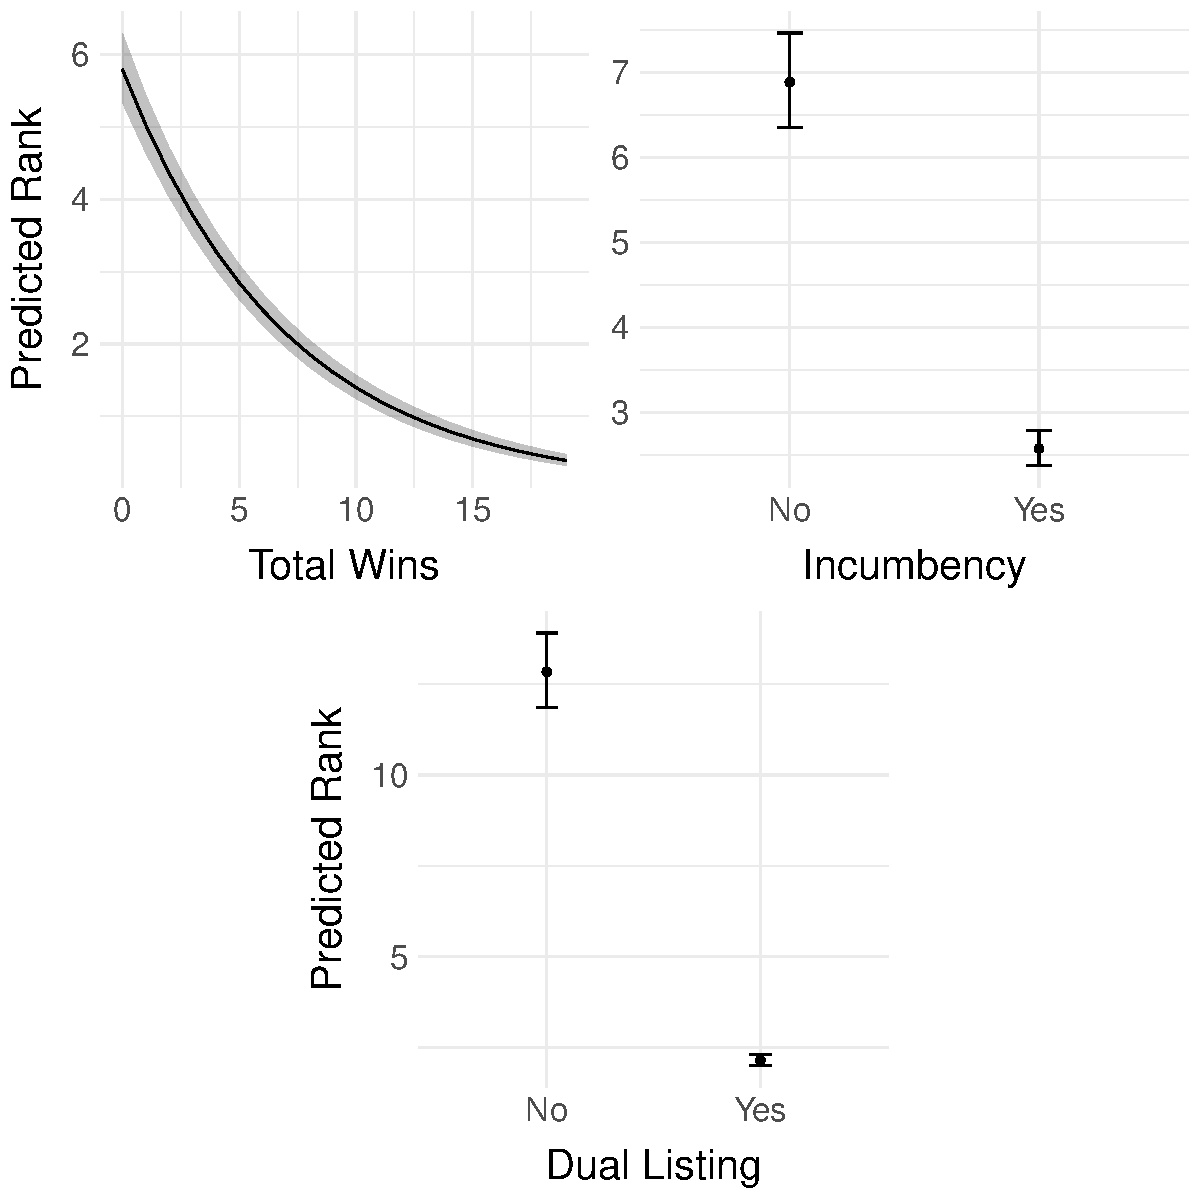
\includegraphics[width = 0.9\textwidth]{../figure/paper/h1_h2_h3.pdf}
	\label{fig:rank}
\end{figure}

\section{Discussion} \label{sec: dis}

\subsection{Youth Underrepresentation Without Dual Listing}

The above result shows a general tendency in Japan's lower house election that parties place dual-listed candidates, senior politicians, and incumbents on higher list positions in the list tier. In addition, returning candidates and those who have served longer in parliament are more likely to be given second chances. Altogether, these findings suggest that parties give insurance tickets to their senior members and incumbents using the option of dual listing. 

What would have happened if parties had not been allowed to take that option? To consider the causal effect of allowing dual listing on youth representation in parliament, one needs to identify whom and how parties would have been nominated in the absence of dual listing. This task is daunting: since we are interested in the effect of an electoral rule, we need to specify the point of divergence, i.e., a point where dual listing had become prohibited, but there are too many possibilities. For example, it could have been at the point of the 1994 electoral reform or later than that. In addition, even if we could specify the starting point of the counterfactual scenario, it would be all the more difficult to consider parties' nomination strategies absent dual listing. Parties can adapt to the external environment: since the 1994 reform, parties in Japan have adapted their strategies to the new electoral rules. It would not be clear what kind of candidates parties had nominated if dual listing had not been allowed. 

However, it would not be unreasonable to partially extrapolate the identities of counterfactual nominees from observed data. Specifically, I consider the age of candidates who would have been nominated absent the dual listing option and claim that young citizens would have been better represented in this situation. Recall that dual listing forces parties into a tradeoff between giving second chances to existing candidates and nominating new candidates. Without dual listing, this dilemma disappears, and parties would replace existing SMD candidates with new candidates whose age would be lower than the average candidate or those they replace. Figure \ref{fig:ageFirstRun} compares the average age of candidates (solid lines) with that of candidates running for the first time (dashed lines) across the two tiers (red) and focusing on the PR tier (blue). In each election, new candidates are about three years younger than the average. Narrowing down to the PR tier, new candidates are about three to five years younger than the average. The same patterns apply when comparing the age of winners to that of those elected for the first time (Figure \ref{fig:ageFirstWin}). 

\begin{figure}[!htbp]
	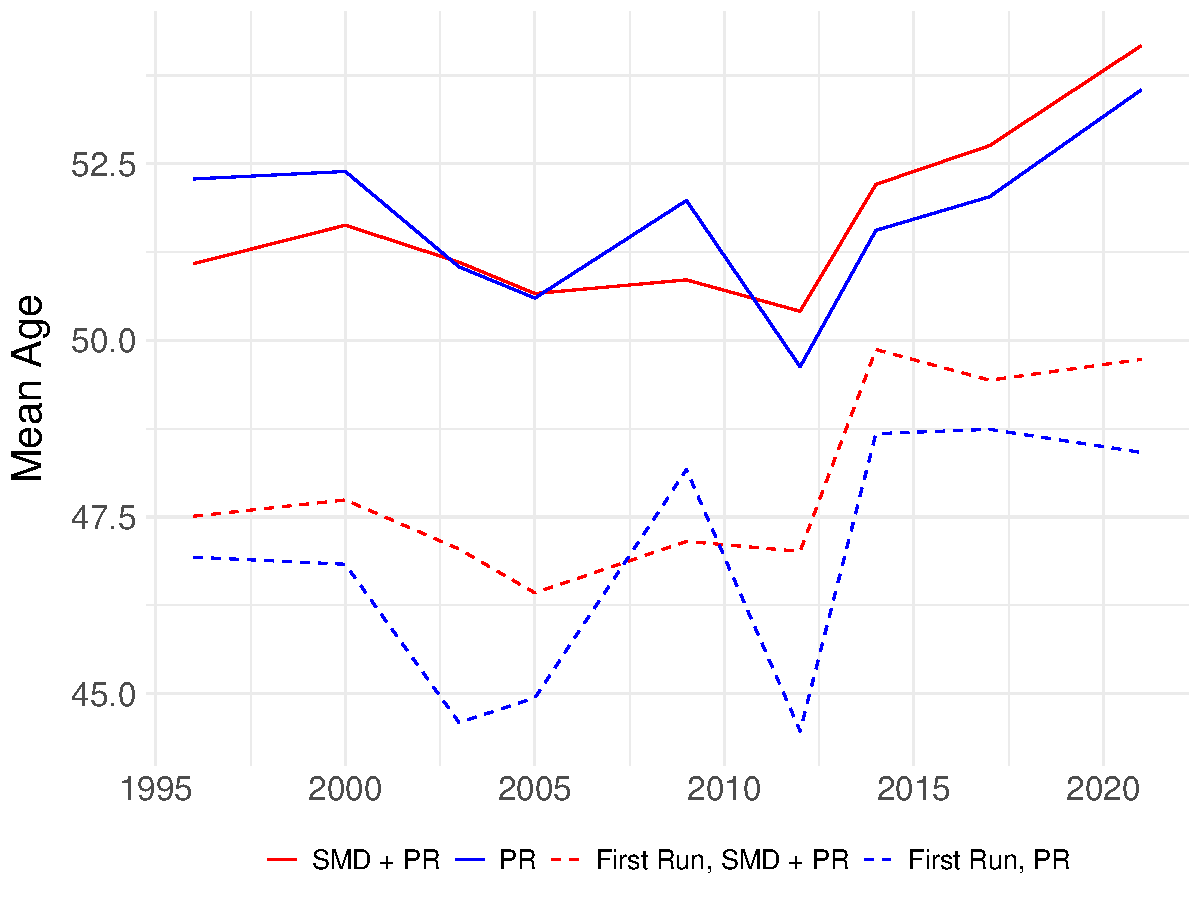
\includegraphics[width = 0.9\textwidth]{../figure/paper/age_first_run.pdf}
	\caption{Age Comparison: Average vs. New Candidates}
	\label{fig:ageFirstRun}
\end{figure}

Since rookie candidates and new MPs are younger than the average, one could reasonably expect that candidates who would have run in the absence of dual listing would have contributed to mitigating youth underrepresentation in parliament. Of course, parties may have adopted a different nomination strategy under this hypothetical scenario. For example, they might have nominated some of the senior candidates and incumbents in the PR tier, where they can expect certain seat gains, and other candidates in the majoritarian tier. However, even in such cases, youth underrepresentation would have been mitigated across the two layers of the system. 

\subsection{General Implications}

This study explores why the PR tier of Japan's mixed-member electoral system underrepresents young citizens to the same extent as the majoritarian tier and argues that the interaction between the two tiers of the system, dual listing, incentivizes parties to give insurance tickets to existing candidates, thus preventing legislative turnover. Analyzing the nomination patterns of candidates in the PR tier of the lower house elections between 1996 and 2017, I first present evidence that parties are more likely to dual-list senior candidates and incumbents than others. Next, I show that these types of candidates, along with dual-listed candidates, tend to be placed higher on the party list. Overall, these results suggest that parties provide higher electoral prospects to existing candidates using dual listing, hindering legislative turnover. Given that new candidates are generally much younger than the candidate or legislative average, the problem of youth underrepresentation would have been mitigated without dual listing. 

Apart from explaining the above puzzle, this research has implications for topics of comparative politics. First, it complements previous cross-national studies that explore the relationship between electoral rules and youth representation by proposing a potential mechanism connecting the two elements. My argument focuses on parties' incentives and behaviors shaped by institutional rules: most parties do not simply attempt to maximize the number of seats but also try to realize their desired policies. To that end, they must send politicians with more experience and resources into parliament. When parties are given opportunities to ensure the election of such candidates, it is reasonable to expect to exploit them. At this time, the ones who become victims are those in the pool of potential candidates. 

The findings of this paper also have implications for studies of electoral systems. Scholars often consider that mixed-member systems combine the advantages of majoritarian and PR electoral systems, thereby achieving the ``best of the both worlds". However, as far as minority representation is concerned, mixed systems can act similarly to majoritarian systems. Minority representation under PR systems crucially depends on how willing parties are to nominate candidates of underrepresented groups. While parties have incentives to do so in pure-PR systems, conflicting rationales may slip in under mixed systems. In the current case, party motivations to represent a broader range of cleavages within society are partially overridden by the incentives to ensure the election of senior legislators. A key takeaway is that the representational advantages of PR systems might be diminished without a proper institutional arrangement under mixed-member systems. 


\newpage

\bibliography{../Reference.bib}
\bibliographystyle{apalike}

\newpage

\appendix

\setcounter{table}{0}
\setcounter{figure}{0}
\renewcommand{\thetable}{A\arabic{table}}
\renewcommand{\thefigure}{A\arabic{figure}}

\section{Summary Statistics}

\subsection{Candidate-Level Summary}

\begin{table}[!htbp] \centering \renewcommand*{\arraystretch}{1.1}\caption{Summary Statistics}\resizebox{\textwidth}{!}{
\begin{threeparttable}
\begin{tabular}{l|cccccccc}
\toprule
Variable & N & Mean / \% & Std. Dev. & Min & \% 25 & \% 50 & \% 75 & Max \\ 
\midrule
Gender & 6935 &  &  &  &  &  &  &  \\ 
... Female & 881 & 12.7\% &  &  &  &  &  &  \\ 
... Male & 6054 & 87.3\% &  &  &  &  &  &  \\ 
N of wins before & 6935 & 1.776 & 2.487 & 0 & 0 & 1 & 3 & 19 \\ 
Incumbency & 6935 &  &  &  &  &  &  &  \\ 
... Incumbent & 3129 & 45.1\% &  &  &  &  &  &  \\ 
... Non-Incumbent & 3806 & 54.9\% &  &  &  &  &  &  \\ 
List Rank & 6935 & 4.317 & 6.976 & 1 & 1 & 2 & 4 & 52\\ 
Dual Listing & 6935 &  &  &  &  &  &  &  \\ 
... Yes & 5292 & 76.3\% &  &  &  &  &  &  \\ 
... No & 1643 & 23.7\% &  &  &  &  &  &  \\ 
\bottomrule
\end{tabular}
\begin{tablenotes}[flushleft]
  \scriptsize{
    \item Candidate-level summary statistics. 
    \item \textit{Data source}: \citet{reedsmith2018} 
  }
\end{tablenotes}
\end{threeparttable}
}
\label{tab:stats}
\end{table}



\newpage

\subsection{Magnitudes of PR Blocks, 1996 - 2017}

% created manually
\begin{table}[!htbp]
\begin{threeparttable}
\begin{tabular}{lccccccccc}
\toprule
Bloc & 1996 & 2000 & 2003 & 2005 & 2009 & 2012 & 2014 & 2017 & 2021 \\
\midrule
Hokkaido & 9 & 8 & 8 & 8 & 8 & 8 & 8 & 8 & 8 \\
Tohoku & 16 & 14 & 14 & 14 & 14 & 14 & 14 & 13 & 13 \\
Kita-kanto & 21 & 20 & 20 & 20 & 20 & 20 & 20 & 19 & 19 \\
Tokyo & 19 & 17 & 17 & 17 & 17 & 17 & 17 & 17 & 17 \\
Minami-kanto & 23 & 21 & 22 & 22 & 22 & 22 & 22 & 22 & 22 \\
Hokuriku Shinetsu & 13 & 11 & 11 & 11 & 11 & 11 & 11 & 11 & 11 \\
Tokai & 23 & 21 & 21 & 21 & 21 & 21 & 21 & 21 & 21 \\
Kinki & 33 & 30 & 30 & 30 & 29 & 29 & 29 & 28 & 28 \\
Chugoku & 13 & 11 & 11 & 11 & 11 & 11 & 11 & 11 & 11 \\
Shikoku & 7 & 6 & 6 & 6 & 6 & 6 & 6 & 6 & 6 \\
Kyushu & 23 & 21 & 21 & 21 & 21 & 21 & 21 & 20 & 20 \\
\bottomrule
\end{tabular}
\begin{tablenotes}[flushleft]
  \scriptsize{
    \item Magnitudes of each PR regional district for elections 1996 - 2021. 
    \item \textit{Data source}: \citet{reedReedSmithJapaneseHouse2017, ministryofinternalaffairsandcommunicationsElectionSenkyo2024}
  }
\end{tablenotes}
\end{threeparttable}
\caption{Magnitudes of PR Blocks}
\label{tab:distM}
\end{table}

\newpage

\subsection{Distribution of List Rank}

\begin{figure}[!htbp]
	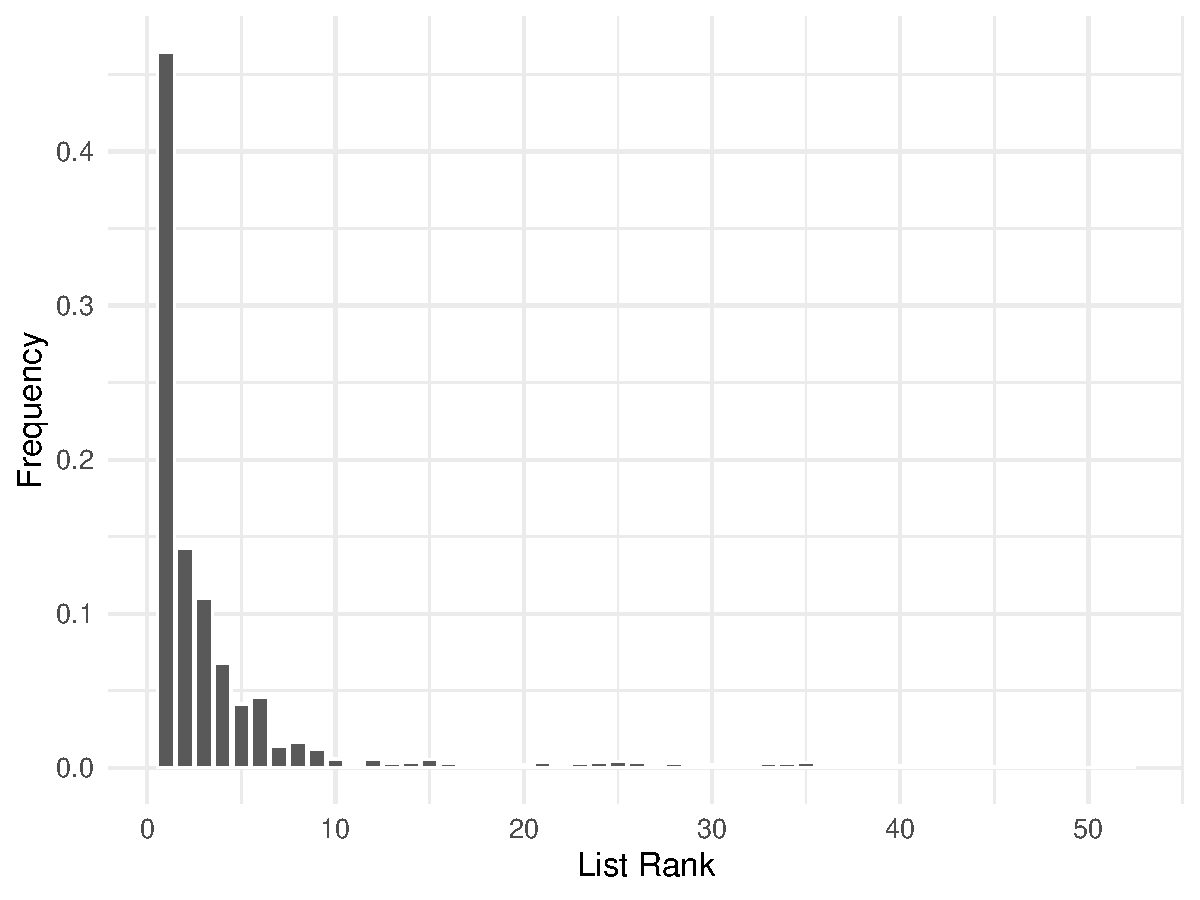
\includegraphics[width = 0.9\textwidth]{../figure/paper/pr_rank_distribution.pdf}
	\caption{Distribution of List Rank}
	\label{fig:distRank}
\end{figure}

\newpage

\subsection{Age of Winners}

\begin{figure}[!htbp]
	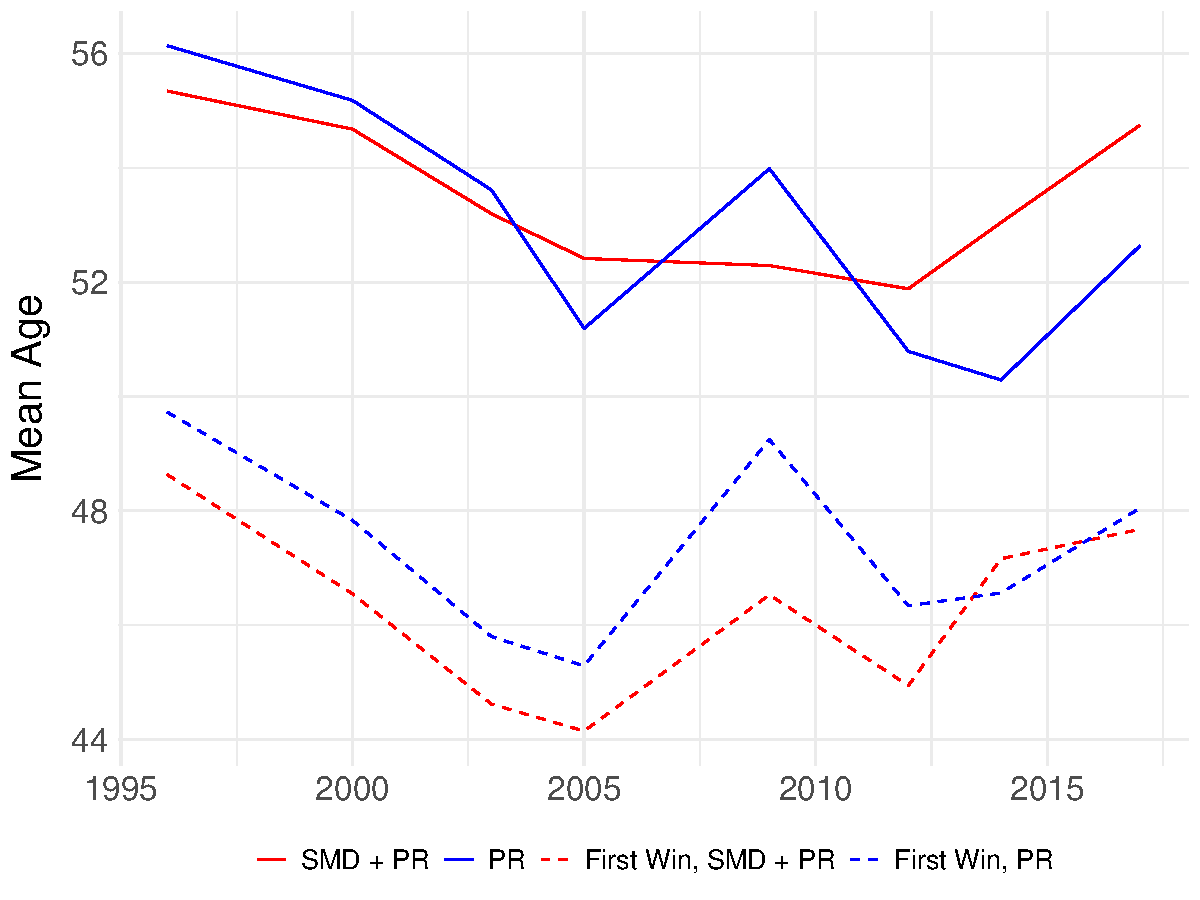
\includegraphics[width = 0.9\textwidth]{../figure/paper/age_first_win.pdf}
	\caption{Age Comparison: Average vs. New Legislators}
	\label{fig:ageFirstWin}
\end{figure}	

\end{document}































